\documentclass[12pt,letterpaper,oneside,reqno]{amsart}
\usepackage{amsfonts}
\usepackage{amsmath}
\usepackage{amssymb}
\usepackage{amsthm}
\usepackage{float}
\usepackage{mathrsfs}
\usepackage{colonequals}
\usepackage[font=small,labelfont=bf]{caption}
\usepackage[pdfpagelabels,hyperindex,colorlinks=true,linkcolor=blue,urlcolor=magenta,citecolor=green]{hyperref}
\usepackage{graphicx}
\emergencystretch=1em
\usepackage{array}
\usepackage{enumitem}
\usepackage{etoolbox}
\usepackage{physics}

% margins and layout
\linespread{1.7}
\usepackage[left=1in,right=1in,bottom=1in,top=1in]{geometry}
\apptocmd{\sloppy}{\hbadness 10000\relax}{}{}
\raggedbottom

\newcommand \coeffA [3][A] {{\mathbf{#1}} \sb{#2,#3}}
\newcommand \polynomialP [4][P]{{\mathbf{#1}}\sp{#2} \sb{#3}(#4)}
\newcommand \bernoulli [2][B] {{#1}\sb{#2}}

% for brack coefficient
\newcommand \brackCoefficient [3] {{#1 \brack #2}_{#3}}
\newcommand \braceCoefficient [3] {{#1 \brace #2}_{#3}}

% free foot note
%\let\svthefootnote\thefootnote
%\newcommand\freefootnote[1]{%
%    \let\thefootnote\relax%
%    \footnotetext{#1}%
%    \let\thefootnote\svthefootnote%
%}


\newtheorem{theorem}{Theorem}[section]
\newtheorem{corollary}[theorem]{Corollary}
\newtheorem{proposition}[theorem]{Proposition}
\newtheorem{observation}[theorem]{Observation}
\newtheorem{lemma}[theorem]{Lemma}
\newtheorem{claim}[theorem]{Claim}
\newtheorem{example}[theorem]{Example}
\newtheorem{conjecture}[theorem]{Conjecture}
\newtheorem{definition}[theorem]{Definition}
\newtheorem{question}[theorem]{Question}
\newtheorem{remark}[theorem]{Remark}
\newtheorem{assumption}[theorem]{Assumption}

\numberwithin{equation}{section}

\title[Surprising Polynomial Identities arising from a Classical Interpolation Problem]
{Surprising Polynomial Identities arising from a Classical Interpolation Problem}
\author[Petro Kolosov]{Petro Kolosov}
%\date{\today}

% metadata
%\email{kolosovp94@gmail.com}
%\address{Software Developer, DevOps Engineer}
%\urladdr{https://kolosovpetro.github.io}
%\subjclass[2010]{26E70, 05A30}
%\keywords{Polynomial identities,
%    Finite differences,
%    Binomial coefficients,
%    Faulhaber's formula,
%    Power sums,
%    Bernoulli numbers,
%    Combinatorics,
%    Pascal's triangle,
%    OEIS}
%\hypersetup{
%    pdftitle={Surprising Polynomial Identities arising from a Classical Interpolation Problem},
%    pdfproducer={LaTeX},
%    pdfcreator={pdflatex},
%    pdfauthor={Petro Kolosov},
%    pdfsubject={New Polynomial Identities Derived via Classical Interpolation Techniques},
%    pdfkeywords={Polynomial identities,
%        Finite differences,
%        Binomial coefficients,
%        Faulhaber's formula,
%        Power sums,
%        Bernoulli numbers,
%        Combinatorics,
%        Pascal's triangle,
%        OEIS}
%}

\begin{document}

    \maketitle

%    \begin{abstract}
%        The polynomial $\mathbf{P}^m_b(x)$ is a polynomial of degree $2m+1$ in $(x,b) \in \mathbb{R}$,
defined by an identity for odd powers, closely linked to Binomial theorem and Faulhaber's formula.

The odd-power identity is derived using certain interpolation techniques,
including systems of linear equations, recurrence formulas, and finite differences.
This manuscript offers a comprehensive historical survey of the milestones and evolution
of the polynomial $\mathbf{P}^m_b(x)$, followed by related works based on it.

Notable results in related works include the relation between ordinary and partial derivatives
for odd powers, finding polynomial derivatives via a double limit, power function approximations,
connection between discrete convolution of power function, dynamic equations on times scales, etc.

Finally, the manuscript proposes future research directions,
along with Mathematica programs to validate intermediate results.

%    \end{abstract}

%    \tableofcontents

%    \freefootnote{Sources: \url{https://github.com/kolosovpetro/surprising-polynomial-identities-classical-interpolation}}


    \section{Discussion on interpolation of cubes}
    \label{sec:the-problem-of-interpolation-of-cubes}
    This is the story of a student with a deep curiosity for mathematics.
Although, not a specialist in mathematics,
our young explorer always possessed a strong sense of mathematical beauty and aesthetics.
The mathematical knowledge of the individual was limited by undergraduate level course, which includes the basics of
matrix operations, basic calculus, and elementary linear algebra.
One day, our student found himself observing the tables of finite differences, precisely finite differences of cubes.

By observing the table
\begin{table}[H]
    \begin{center}
        \setlength\extrarowheight{-6pt}
        \begin{tabular}{c|cccc}
            $n$ & $n^3$ & $\Delta(n^3)$ & $\Delta^2(n^3)$ & $\Delta^3(n^3)$ \\
            \hline
            0   & 0     & 1             & 6               & 6               \\
            1   & 1     & 7             & 12              & 6               \\
            2   & 8     & 19            & 18              & 6               \\
            3   & 27    & 37            & 24              & 6               \\
            4   & 64    & 61            & 30              & 6               \\
            5   & 125   & 91            & 36              &                 \\
            6   & 216   & 127           &                 &                 \\
            7   & 343   &               &                 &
        \end{tabular}
    \end{center}
    \caption{Table of finite differences of the polynomial $n^3$.} \label{tab:table}
\end{table}

The first question that visited curious mind was
\begin{question}
    \label{quest:interpolation-cubes}
    How to reconstruct the value of $n^3$ from its finite differences?
\end{question}
Precisely, the inquiry is to find a way to reconstruct the values of the sequence $\{0, 1, 8, 27, 64, \ldots\}$
given the values of finite differences in the table.

In its essence, the problem is so old that it can be traced back to ancient Babylonian and Greek times,
several centuries BC and first centuries AD~\cite{gautschi2012interpolation}.
The process of finding new data points based on the range of a discrete set
of known data points is called interpolation.
Interpolation, as we know it today, was developed in 1674--1684 by Isaac Newton
in his works referenced as foundation of classical interpolation theory~\cite{meijering2002chronology}.
For instance, Newton's series for $n^3$ is
\begin{align*}
    n^3 = 6 \binom{n}{3} + 6\binom{n}{2} + 1 \binom{n}{1} + 0\binom{n}{0}
\end{align*}
because $f(x) = \sum_{k=0}^{d} \Delta^{d-k} f(0) \binom{x}{d-k}$, see~\cite[~p. 190]{graham1994concrete}.

Great!
But there is one thing, the student who has risen the question~\eqref{quest:interpolation-cubes}
had no clue about interpolation theory at all.
What he decided then?
Exactly, he decided to try to re-invent interpolation formula himself,
fueled by the purest feeling of mystery.
His mind was occupied by only a single thought:
\textit{All mathematical truths exist timelessly, we only reveal and describe them.}
That mindset inspired our student to start his own mathematical journey.

By observing the table of finite differences~\eqref{tab:finite-differences-cubes} we can notice that
the first order finite difference of cubes may be expressed in terms of its
third order finite difference $\Delta^3(n^3) = 6$, as follows
\begin{align*}
    \begin{split}
        \Delta(0^3) &= 1+6 \cdot 0 \\
        \Delta(1^3) &= 1+6\cdot0+6\cdot1 \\
        \Delta(2^3) &= 1+6\cdot0+6\cdot1+6\cdot2 \\
        \Delta(3^3) &= 1+6\cdot0+6\cdot1+6\cdot2+6\cdot3 \\
        &\; \; \vdots \\
        \Delta(n^3) &= 1+6\cdot0+6\cdot1+6\cdot2+6\cdot3 + \cdots + 6n
    \end{split}
\end{align*}
By using sigma notation, we get
\begin{align*}
    \Delta(n^3) = 1+6\cdot0+6\cdot1+6\cdot2+6\cdot3+\cdots+6\cdot n = 1 + 6 \sum_{k=0}^{n} k
\end{align*}

However, there is a more beautiful way to prove that $\Delta(n^3) = 1 + 6 \sum_{k=0}^{n} k$.
We refer to one of the finest articles in the area of polynomials and power sums,
that is \textit{Johann Faulhaber and sums of powers} written by Donald Knuth~\cite{knuth1993johann}.
Indeed, this article is a great source to reach piece of mind in mathematics.
We now focus on the odd power identities shown at~\cite[~p. 9]{knuth1993johann}
\begin{align*}
    n^1 &= \binom{n}{1} \\
    n^3 &= 6 \binom{n+1}{3} + \binom{n}{1} \\
    n^5 &= 120 \binom{n+2}{5} + 30 \binom{n+1}{3} + \binom{n}{1}
\end{align*}

It is quite interesting that the identity in terms of triangular numbers $\binom{n+1}{2}$
and finite differences of cubes becomes more obvious
\begin{align*}
    \Delta n^3
    = (n+1)^3 - n^3
    =  6 \binom{n+1}{2} + \binom{n}{0}
\end{align*}
It easy to see that
\begin{align*}
    \Delta n^3
    = \left[ 6 \binom{n+2}{3} + \binom{n+1}{1} \right] - \left[ 6 \binom{n+1}{3} + \binom{n}{1} \right]
    = 6 \binom{n+1}{2} + \binom{n}{0}
\end{align*}
because $\binom{n}{k} = \binom{n-1}{k} + \binom{n-1}{k-1}$.

Moreover, the concept above allows to reach $N$-fold power sums $\sum^N k^{2m+1}$
or finite differences $\Delta^N k^{2m+1}$ of odd powers by simply altering
binomial coefficients indexes.
Quite strong and impressive.

We can observe that triangular numbers $\binom{n+1}{2}$ are equivalent to
\begin{align*}
    \binom{n+1}{2} = \sum_{k=0}^{n} k
\end{align*}
because $\binom{n+1}{m+1} = \sum_{k=0}^{n} \binom{k}{m}$.
This leads to the identity in finite differences of cubes
\begin{align*}
    \Delta n^3 = (n+1)^3 - n^3 = 1 + 6 \sum_{k=0}^{n} k
\end{align*}
An experienced mathematician would immediately notice a spot to apply Faulhaber's formula~\cite{beardon1996sums}
to get the closed form of the sum $\sum_{k=0}^{n} k$
\begin{align*}
    \sum_{k=0}^{n} k = \frac{1}{2}(n+n^2)
\end{align*}
Thus, the finite difference $\Delta(n^3)$ takes a well-known form,
which matches Binomial theorem~\cite{abramowitz1988handbook}
\begin{align*}
    \Delta(n^3)
    = 1 + 6 \left[ \frac{1}{2}(n+n^2) \right]
    = 1 + 3 n + 3 n^2
    = \sum_{k=0}^{2} \binom{3}{k} n^k
\end{align*}
And\ldots that could be the end of the story, isn't it?
Because all what remains is to say that
\begin{align*}
    n^3
    = \sum_{k=0}^{n-1} (k+1)^3 - k^3
    = \sum_{k=0}^{n-1} \left( 1 + 6 \sum_{t=0}^{k} t \right)
    = \sum_{k=0}^{n-1} 1 + 3 k + 3 k^2
\end{align*}
Thus, the polynomial $n^3$ is interpolated successfully, and thus,
our protégée's question~\eqref{quest:interpolation-cubes} is answered positively.
Because we have successfully found the function that matches $n^3$ from the values of its finite differences from the
table~\eqref{tab:finite-differences-cubes}.

However, not this time.
Luckily enough (say), the student who has stated the question~\eqref{quest:interpolation-cubes}
wasn't really aware of the approaches above neither.
What a lazy student!
Probably, that's exactly the case when unawareness leads to a fresh sight to century-old questions,
leading to unexpected results and new insights.
Instead, our investigator spotted a little bit different pattern in $\Delta n^3= 6 \binom{n+1}{2} + \binom{n}{0}$.

Consider the polynomial $n^3$ as sum of its finite differences
\begin{align*}
    n^3
    &= [1+6\cdot0] \\
    &+ [1+6\cdot0+6\cdot1] \\
    &+ [1+6\cdot0+6\cdot1+6\cdot2] + \cdots \\
    &+ [1+6\cdot0+6\cdot1+6\cdot2+\cdots+6\cdot(n-1)]
\end{align*}
We can observe that the term $1$ appears $n$ times, the item $6\cdot0$ appears $n-0$ times,
the item $6\cdot1$ appears $n-1$ times and so on.
By rearranging recurring common terms
\begin{align*}
    n^3 = n
    &+ [(n-0) \cdot 6 \cdot 0] \\
    &+ [(n-1)\cdot6\cdot1] \\
    &+ [(n-2)\cdot6\cdot2] + \cdots \\
    &+ [(n-k)\cdot 6 \cdot k] + \cdots \\
    &+ [1\cdot6\cdot(n-1)]
\end{align*}
By applying compact sigma sum notation yields an identity for cubes $n^3$
\begin{align*}
    n^3 = n + \sum_{k=0}^{n-1} 6k(n-k)
\end{align*}
We can freely move the term $n$ under the summation because there are exactly $n$ iterations.
Therefore,
\begin{align*}
    n^3 = \sum_{k=0}^{n-1} 6k(n-k) + 1
\end{align*}
By inspecting the expression $6k(n-k) + 1$, we can notice that it is symmetric over $k$.
Let be $T_{1} (n,k) = 6k(n-k) + 1$ then
\begin{align*}
    T_{1} (n,k) = T_{1} (n,n-k)
\end{align*}
This symmetry allows us to alter summation bounds easily.
Hence,
\begin{align*}
    n^3 = \sum_{k=1}^{n} 6k(n-k) + 1
\end{align*}
By arranging the values of $T_{1} (n,k)$ as a triangular array, we see that cube identities indeed are true
\begin{table}[H]
    \setlength\extrarowheight{-6pt}
    \begin{tabular}{c|cccccccc}
        $n/k$ & 0 & 1  & 2  & 3  & 4  & 5  & 6  & 7 \\
        \hline
        0     & 1 &    &    &    &    &    &    &   \\
        1     & 1 & 1  &    &    &    &    &    &   \\
        2     & 1 & 7  & 1  &    &    &    &    &   \\
        3     & 1 & 13 & 13 & 1  &    &    &    &   \\
        4     & 1 & 19 & 25 & 19 & 1  &    &    &   \\
        5     & 1 & 25 & 37 & 37 & 25 & 1  &    &   \\
        6     & 1 & 31 & 49 & 55 & 49 & 31 & 1  &   \\
        7     & 1 & 37 & 61 & 73 & 73 & 61 & 37 & 1
    \end{tabular}
    \caption{Values of $T(n,k) = 6k(n-k) + 1$.
    See the sequence \href{https://oeis.org/A287326}{\texttt{A287326}} in OEIS
    ~\cite{oeis_numerical_triangle_row_sums_give_cubes}.}
    \label{tab:triangle_row_sums_give_cubes}
\end{table}

The following recurrence holds for $T_{1} (n,k)$
\begin{align*}
    T_{1} (n, k) = 2T_{1} (n-1, k) - T_{1} (n-2, k)
\end{align*}
Which is indeed true, because
\begin{align*}
    T_{1} (5, 2) = 2 \cdot 25 - 13 = 37
\end{align*}
Finally, our curious learner has reached the first milestone, by finding his own
answer to the question~\eqref{quest:interpolation-cubes} and the answer was positive.
What an excitement it was!
However, it wouldn't take long.
Indeed, curiosity is not something that can be fulfilled completely,
and thus new questions arise.
Somehow, the inquirer got a strong feeling that something bigger, something even more general
hides behind the identity $n^3 = \sum_{k=1}^{n} 6k(n-k) + 1$.
That was quite intuitive.
Fair enough that the next question was
\begin{question}
    Given that the identity $n^3 = \sum_{k=1}^{n} 6k(n-k) + 1$ holds for the polynomial $n^3$,
    can it be extended or generalized to higher-degree powers, such as $n^4$ or $n^5$,
    in a similar manner?
    \label{question:higher_powers}
\end{question}

However, this time it was not so easy for the young explorer to find identity for $n^4$ or $n^5$
by simply observing the tables of finite differences.
The previous approach to express the difference of cubes $\Delta n^3$ in terms of
$\Delta^3 n^3 = 6$ and then express the cubes as $n^3 = \sum_k 6k (n-k) +1$ --- was not successful.
Moreover, it wasn't even clear what is the generic form of an identity our student was looking for,
a lot of concerns came from a simple interpolation task.
Thus, the question~\eqref{question:higher_powers} was shared with the mathematical community.
And there was an answer.


    \section{A system of linear equations}
    \label{sec:system-of-linear-equations-approach}
    In 2018, Albert Tkaczyk published two papers~\cite{tkaczyk2018problem, tkaczyk2018continuation}
presenting analogous identities for polynomials $n^5, \; n^7$ and $n^9$
derived in a manner similar to $n^3 = \sum_{k=1}^{n} 6k(n-k) + 1$.
Tkaczyk assumed that the identity for $n^5$ takes the following explicit form
\begin{align*}
    n^5 = \sum_{k=1}^{n} \left[ A k^2(n-k)^2 + Bk(n-k) + C \right]
\end{align*}
where $A,B,C$ are yet-unknown coefficients.
We denote $A,B,C$ as $\coeffA{2}{0}, \coeffA{2}{1}, \coeffA{2}{2}$
to reach the compact form of double sum
\begin{align*}
    n^5 = \sum_{k=1}^{n} \sum_{r=0}^{2} \coeffA{2}{r} k^r (n-k)^r
\end{align*}
By observing the equation above, the potential form of generalized odd-power identity becomes more obvious.
One important note to add here, we define $0^x = 1$ for all $x$, see~\cite[~p. 162]{graham1994concrete}.
This is because when $k=n$ and $r=0$ the term $k^r (n-k)^r = n^0 \cdot 0^0$, thus we must define $0^x = 1$
for all $x$.

To evaluate the set of coefficients $\coeffA{2}{0}, \coeffA{2}{1}, \coeffA{2}{2}$
we construct and solve a certain system of linear equations, which is
built as follows
\begin{align*}
    n^5 = \coeffA{2}{0} \sum_{k=1}^{n} k^0 (n-k)^0 + \coeffA{2}{1} \sum_{k=1}^{n} k^1 (n-k)^1 + \coeffA{2}{2} \sum_{k=1}^{n} k^2 (n-k)^2
\end{align*}
By expanding the sums $\sum_{k=1}^{n} k^r (n-k)^r$ using Faulhaber's formula~\cite{beardon1996sums}, we get
an equation
\begin{equation*}
    \coeffA{2}{0} n
    + \coeffA{2}{1} \left[ \frac{1}{6} (n^3-n) \right]
    + \coeffA{2}{2} \left[ \frac{1}{30} (n^5-n) \right] - n^5 = 0
\end{equation*}
By multiplying by $30$ both right-hand side and left-hand side, we get
\begin{equation*}
    30 \coeffA{2}{0} n + 5 \coeffA{2}{1} (n^3-n) + \coeffA{2}{2} (n^5-n) - 30n^5 = 0
\end{equation*}
By expanding the brackets and rearranging the terms
\begin{equation*}
    30 \coeffA{2}{0} - 5 \coeffA{2}{1} n + 5 \coeffA{2}{1} n^3 - \coeffA{2}{2} n + \coeffA{2}{2} n^5 - 30n^5 = 0
\end{equation*}
By combining the common terms, we obtain
\begin{equation*}
    n (30 \coeffA{2}{0} - 5 \coeffA{2}{1} - \coeffA{2}{2}) + 5 \coeffA{2}{1} n^3 + n^5 (\coeffA{2}{2} - 30) = 0
\end{equation*}
Therefore,
\begin{equation*}
    \begin{cases}
        30 \coeffA{2}{0} - 5 \coeffA{2}{1} - \coeffA{2}{2} &= 0 \\
        \coeffA{2}{1} &= 0 \\
        \coeffA{2}{2} - 30 &= 0
    \end{cases}
\end{equation*}
By solving the system above, we evaluate the coefficients $\coeffA{2}{0}, \coeffA{2}{1}, \coeffA{2}{2}$
\begin{equation*}
    \begin{cases}
        \coeffA{2}{2} &= 30 \\
        \coeffA{2}{1} &= 0 \\
        \coeffA{2}{0} &= 1
    \end{cases}
\end{equation*}
Thus, the identity for $n^5$
\begin{equation*}
    n^5 = \sum_{k=1}^{n} 30k^2(n-k)^2 + 1
\end{equation*}
Again, the terms $30k^2(n-k)^2 + 1$ are symmetric over $k$.
Let be $T_2 (n,k) = 30k^2(n-k)^2 + 1$ then
\begin{align*}
    T_2 (n,k) = T_2 (n,n-k)
\end{align*}
By arranging the values of $T_{2} (n,k)$ as a triangular array, we see that the identity for $n^5$ is indeed true
\begin{table}[H]
    \setlength\extrarowheight{-6pt}
    \begin{tabular}{c|cccccccc}
        $n/k$ & 0 & 1    & 2    & 3    & 4    & 5    & 6    & 7 \\
        \hline
        0     & 1 &      &      &      &      &      &      &   \\
        1     & 1 & 1    &      &      &      &      &      &   \\
        2     & 1 & 31   & 1    &      &      &      &      &   \\
        3     & 1 & 121  & 121  & 1    &      &      &      &   \\
        4     & 1 & 271  & 481  & 271  & 1    &      &      &   \\
        5     & 1 & 481  & 1081 & 1081 & 481  & 1    &      &   \\
        6     & 1 & 751  & 1921 & 2431 & 1921 & 751  & 1    &   \\
        7     & 1 & 1081 & 3001 & 4321 & 4321 & 3001 & 1081 & 1
    \end{tabular}
    \caption{Values of $30k^2(n-k)^2 + 1$.
    See the OEIS entry \href{https://oeis.org/A300656}{\texttt{A300656}}
    ~\cite{oeis_numerical_triangle_row_sums_give_fifth_powers}.}
    \label{tab:row-sums-gives-fifth-power}
\end{table}

The following recurrence holds for $T_2 (n,k)$
\begin{align*}
    T_2 (n, k) = 3T_2(n-1, k) - 3T_2(n-2, k) + T_2(n-3, k)
\end{align*}
Which is indeed true because
\begin{align*}
    T_2 (6,2) = 3 \cdot 1081 - 3 \cdot 481 + 271 = 1921
\end{align*}

%Consider an example for $n^7$.
%\begin{align*}
%    n^7 =
%    \coeffA{3}{0} n
%    + \coeffA{3}{1} \left[ \frac{1}{6} (n^3-n) \right]
%    &+ \coeffA{3}{2} \left[ \frac{1}{30} (n^5-n) \right] \\
%    &+ \coeffA{3}{3} \left[ \frac{1}{420} (3n^7+7n^3-10n) \right]
%\end{align*}
%By multiplying by $30$ both right-hand side and left-hand side, we get
%\begin{align*}
%    420 \coeffA{3}{0} n + 70 \coeffA{2}{1} (n^3-n)
%    &+ 14 \coeffA{2}{2} (n^5-n) \\
%    &+ \coeffA{3}{3} (3n^7+7n^3-10n) - 420n^7 = 0
%\end{align*}
%By expanding the brackets and rearranging terms, we obtain
%\begin{align*}
%    420 \coeffA{3}{0} n
%    &- 70 \coeffA{3}{1} + 70 \coeffA{3}{1} n^3 - 14 \coeffA{3}{2} n + 14 \coeffA{3}{2} n^5 \\
%    &- 10 \coeffA{3}{3} n + 7 \coeffA{3}{3} n^3 + 3 \coeffA{3}{3} n^7 - 420n^7 = 0
%\end{align*}
%Combining the common terms yields
%\begin{align*}
%    n (420 \coeffA{3}{0} - 70 \coeffA{3}{1} - 14 \coeffA{3}{2} - 10 \coeffA{3}{3})
%    &+ n^3 (70 \coeffA{3}{1} + 7 \coeffA{3}{3}) \\
%    &+ n^5 14 \coeffA{3}{2}
%    + n^7 (3 \coeffA{3}{3} - 420)
%    = 0
%\end{align*}
%Therefore, we receive the following system of linear equations
%\begin{align*}
%    \begin{cases}
%        420 \coeffA{3}{0} - 70 \coeffA{3}{1} - 14 \coeffA{3}{2} - 10 \coeffA{3}{3} &= 0 \\
%        70 \coeffA{3}{1} + 7 \coeffA{3}{3} &= 0 \\
%        \coeffA{3}{2} - 30 &= 0 \\
%        3 \coeffA{3}{3} - 420 &= 0
%    \end{cases}
%\end{align*}
%By solving it for $\coeffA{3}{0}, \coeffA{3}{1}, \coeffA{3}{2}, \coeffA{3}{3}$, we obtain
%\begin{equation*}
%    \begin{cases}
%        \coeffA{3}{3} &= 140 \\
%        \coeffA{3}{2} &= 0 \\
%        \coeffA{3}{1} = -\frac{7}{70} \coeffA{3}{3} &= -14 \\
%        \coeffA{3}{0} = \frac{(70 \coeffA{3}{1} + 10 \coeffA{3}{3})}{420} &= 1
%    \end{cases}
%\end{equation*}
%Therefore, the identity for $n^7$ holds
%\begin{equation*}
%    n^7 = \sum_{k=1}^{n} 140 k^3 (n-k)^3 - 14k(n-k) + 1
%\end{equation*}
%The values of $140 k^3 (n-k)^3 - 14k(n-k) + 1$ are symmetric over $k$.
%Let be $T_3 (n,k) = 140 k^3 (n-k)^3 - 14k(n-k) + 1$ then
%\begin{align*}
%    T_3 (n,k) = T_3 (n, n-k)
%\end{align*}
%By arranging the values of $T_{3} (n,k)$ as a triangular array, we see that the identity for $n^7$ is indeed true
%\begin{table}[H]
    \setlength\extrarowheight{-6pt}
    \begin{tabular}{c|cccccccc}
        $n/k$ & 0 & 1     & 2      & 3      & 4      & 5      & 6     & 7 \\
        \hline
        0     & 1 &       &        &        &        &        &       &   \\
        1     & 1 & 1     &        &        &        &        &       &   \\
        2     & 1 & 127   & 1      &        &        &        &       &   \\
        3     & 1 & 1093  & 1093   & 1      &        &        &       &   \\
        4     & 1 & 3739  & 8905   & 3739   & 1      &        &       &   \\
        5     & 1 & 8905  & 30157  & 30157  & 8905   & 1      &       &   \\
        6     & 1 & 17431 & 71569  & 101935 & 71569  & 17431  & 1     &   \\
        7     & 1 & 30157 & 139861 & 241753 & 241753 & 139861 & 30157 & 1
    \end{tabular}
    \caption{Values of $140 k^3 (n-k)^3 - 14k(n-k) + 1$.
    See the OEIS entry \href{https://oeis.org/A300785}{\texttt{A300785}}
    ~\cite{oeis_numerical_triangle_row_sums_give_seventh_powers}.}
    \label{tab:row-sums-gives-seventh-power}
\end{table}

%The following recurrence holds for $T_{3} (n,k)$
%\begin{align*}
%    T_{3} (n, k) = 4T_{3} (n-1, k) - 6T_{3} (n-2, k) + 4T_{3} (n-3, k) - T_{3} (n-4, k)
%\end{align*}
%Which is true indeed because
%\begin{align*}
%    T_{3} (7, 1) = 4 \cdot 17431 -6 \cdot 8905 + 4 \cdot 3739 - 1 \cdot 1093 = 30157
%\end{align*}


    \section{Recurrence relation}
    \label{sec:recurrence-relation-approach}
    In 2018, the recurrence relation~\cite{alekseyev2018mathoverflow} that evaluates the coefficients $\coeffA{m}{r}$ for
non-negative integer $m$ was provided by Max Alekseyev, George Washington University.
The main idea of Alekseyev's approach was to utilize a recurrence relation to evaluate the set of coefficients $\coeffA{m}{r}$
starting from the base case $\coeffA{m}{m}$ and then evaluating the next coefficient $\coeffA{m}{m-1}$
recursively, and so on up to $\coeffA{m}{0}$.
We utilize Binomial theorem $(n-k)^r=\sum_{t=0}^{r} (-1)^t \binom{r}{t} n^{r-t} k^t$ and a specific version
of Faulhaber's formula~\cite{beardon1996sums}
\begin{align*}
    \sum_{k=1}^{n} k^{p}
    = \frac{1}{p+1}\sum_{j=0}^{p} \binom{p+1}{j} \bernoulli{j} n^{p+1-j}
    &= \frac{1}{p+1} \left[ \sum_{j=0}^{p+1} \binom{p+1}{j} \bernoulli{j} n^{p+1-j} \right] - \frac{\bernoulli{p+1}}{p+1} \\
    &= \frac{1}{p+1} \left[ \sum_{j} \binom{p+1}{j} \bernoulli{j} n^{p+1-j} \right] - \frac{\bernoulli{p+1}}{p+1}
\end{align*}
The reason we use modified version of Faulhaber's formula is because we want to omit summation bounds, for simplicity.
This helps us to collapse the common terms across complex sums, see also~\cite[~p. 2]{knuth1992two}.
Therefore, we expand the sum $\sum_{k=1}^{n} k^{r} (n-k)^{r}$ using Binomial theorem
\begin{align*}
    \sum_{k=1}^{n} k^{r} (n-k)^{r} = \sum_{t=0}^{r} (-1)^t \binom{r}{t} n^{r-t} \sum_{k=1}^{n} k^{t+r}
\end{align*}
By applying Faulhaber's formula above, we obtain
\begin{align*}
    \sum_{k=1}^{n} k^{r} (n-k)^{r}
    = \sum_{t=0}^{r} (-1)^t \binom{r}{t} n^{r-t} \left[ \left( \frac{1}{t+r+1} \sum_{j} \binom{t+r+1}{j} \bernoulli{j} n^{t+r+1-j} \right) - \frac{\bernoulli{t+r+1}}{t+r+1} \right]
\end{align*}
By moving the common term $\frac{(-1)^t}{t+r+1}$ out of brackets
\begin{align*}
    \sum_{k=1}^{n} k^{r} (n-k)^{r}
    = \sum_{t=0}^{r} \binom{r}{t} \frac{(-1)^t}{t+r+1} \left[ \sum_{j} \binom{t+r+1}{j} \bernoulli{j} n^{2r+1-j} - \bernoulli{t+r+1} n^{r-t} \right]
\end{align*}
By expanding the brackets
\begin{align*}
    \sum_{k=1}^{n} k^{r} (n-k)^{r}
    &= \left[ \sum_{t=0}^{r} \binom{r}{t} \frac{(-1)^t}{t+r+1} \sum_{j} \binom{t+r+1}{j} \bernoulli{j} n^{2r+1-j}  \right] \\
    &- \left[ \sum_{t=0}^{r} \binom{r}{t} \frac{(-1)^t}{t+r+1} \bernoulli{t+r+1} n^{r-t} \right]
\end{align*}
By moving the sum in $j$ and omitting summation bounds in $t$
\begin{align*}
    \sum_{k=1}^{n} k^{r} (n-k)^{r}
    = \left[ \sum_{j, t} \binom{r}{t} \frac{(-1)^t}{t+r+1} \binom{t+r+1}{j} \bernoulli{j} n^{2r+1-j}  \right]
    - \left[ \sum_{t} \binom{r}{t} \frac{(-1)^t}{t+r+1} \bernoulli{t+r+1} n^{r-t} \right]
\end{align*}
By rearranging the sums we obtain
\begin{align}
    \label{eq:rearranging-terms}
    \sum_{k=1}^{n} k^{r} (n-k)^{r}
    &= \left[ \sum_{j} \bernoulli{j} n^{2r+1-j} \sum_{t} \binom{r}{t} \frac{(-1)^t}{t+r+1} \binom{t+r+1}{j}  \right] \\
    &- \left[ \sum_{t} \binom{r}{t} \frac{(-1)^t}{t+r+1} \bernoulli{t+r+1} n^{r-t} \right] \nonumber
\end{align}
We can notice that
\begin{lemma}
    \label{cor:combinatorial-identity}
    For integers $r, j$
    \begin{align*}
        \sum_{t} \binom{r}{t} \frac{(-1)^t}{r+t+1} \binom{r+t+1}{j}
        =\begin{cases}
             \frac{1}{(2r+1) \binom{2r}r} & \text{if } j=0\\
             \frac{(-1)^r}{j} \binom{r}{2r-j+1} & \text{if } j>0
        \end{cases}
    \end{align*}
    \begin{proof}
        An elegant proof is done by Markus Scheuer in~\cite{scheuer2023mathstackexchange}.
    \end{proof}
\end{lemma}
In particular, the sum in lemma~\eqref{cor:combinatorial-identity} is zero for $0< j \leq r$.
To utilize the lemma~\eqref{cor:combinatorial-identity}, we have to move $j=0$ out of summation
in~\eqref{eq:rearranging-terms} to avoid division by zero in $\frac{(-1)^r}{j}$.
Therefore,
\begin{equation*}
    \begin{split}
        \sum_{k=1}^{n} k^{r} (n-k)^{r}
        &= \frac{1}{(2r+1) \binom{2r}r} n^{2r+1}
        + \left[ \sum_{j = 1}^{\infty} \bernoulli{j} n^{2r+1-j} \sum_{t} \binom{r}{t} \frac{(-1)^t}{t+r+1} \binom{t+r+1}{j} \right] \\
        &- \left[ \sum_{t} \binom{r}{t} \frac{(-1)^t}{t+r+1} \bernoulli{t+r+1} n^{r-t} \right]
    \end{split}
\end{equation*}
Hence, we simplify the equation~\eqref{eq:rearranging-terms} by using lemma~\eqref{cor:combinatorial-identity}
\begin{equation*}
    \begin{split}
        \sum_{k=1}^{n} k^{r} (n-k)^{r}
        &= \frac{1}{(2r+1) \binom{2r}r} n^{2r+1}
        + \underbrace{\left[ \sum_{j = 1}^{\infty} \frac{(-1)^r}{j} \binom{r}{2r-j+1} \bernoulli{j} n^{2r-j+1} \right]}_{(\star)} \\
        &- \underbrace{\left[ \sum_{t} \binom{r}{t} \frac{(-1)^t}{t+r+1} \bernoulli{t+r+1} n^{r-t} \right]}_{(\diamond)}
    \end{split}
\end{equation*}
By introducing $\ell=2r-j+1$ to $(\star)$ and $\ell=r-t$ to $(\diamond)$
we collapse the common terms across two sums
\begin{equation*}
    \begin{split}
        \sum_{k=1}^{n} k^{r} (n-k)^{r}
        &= \frac{1}{(2r+1) \binom{2r}r} n^{2r+1}
        + \left[ \sum_{\ell} \frac{(-1)^r}{2r+1-\ell} \binom{r}{\ell} \bernoulli{2r+1-\ell} n^{\ell} \right] \\
        &- \left[ \sum_{\ell} \binom{r}{\ell} \frac{(-1)^{r-\ell}}{2r+1-\ell} \bernoulli{2r+1-\ell} n^{\ell} \right]\\
        &= \frac{1}{(2r+1) \binom{2r}r} n^{2r+1} + 2 \sum_{\mathrm{odd \; \ell}} \frac{(-1)^r}{2r+1-\ell} \binom{r}{\ell} \bernoulli{2r+1-\ell} n^{\ell}
    \end{split}
\end{equation*}
Assuming that $\coeffA{m}{r}$ is defined by the odd-power identity in~\eqref{conj:odd-power-identity},
we obtain the following relation for polynomials in $n$
\begin{equation*}
    \sum_{r=0}^{m} \coeffA{m}{r} \frac{1}{(2r+1) \binom{2r}r} n^{2r+1}
    + 2 \sum_{r=0}^{m} \sum_{\mathrm{odd \; \ell}} \coeffA{m}{r} \frac{(-1)^r}{2r+1-\ell} \binom{r}{\ell} \bernoulli{2r+1-\ell} n^{\ell}
    \equiv n^{2m+1}
\end{equation*}
Replacing odd $\ell$ by $\ell = 2k+1$ we get
\begin{align*}
    \sum_{r=0}^{m} \coeffA{m}{r} \frac{1}{(2r+1) \binom{2r}{r}} n^{2r+1} + 2 \sum_{r=0}^{m} \sum_{k=0}^{\infty} \coeffA{m}{r} \frac{(-1)^r}{2r-2k} \binom{r}{2k+1} \bernoulli{2r-2k} n^{2k+1}  \equiv n^{2m+1}
\end{align*}
By simplifying the term $2$
\begin{align}
    \label{eq:main_relation}
    \sum_{r=0}^{m} \coeffA{m}{r} \frac{1}{(2r+1) \binom{2r}{r}} n^{2r+1} + \sum_{r=0}^{m} \sum_{k=0}^{\infty} \coeffA{m}{r} \frac{(-1)^r}{r-k} \binom{r}{2k+1} \bernoulli{2r-2k} n^{2k+1}  \equiv n^{2m+1}
\end{align}
Basically, the relation~\eqref{eq:main_relation} is the generating function we utilize to
evaluate the values of $\coeffA{m}{0}, \coeffA{m}{1}, \ldots, \coeffA{m}{m}$.
We now fix the unused values of $\coeffA{m}{r}$ so that $\coeffA{m}{r} = 0$ for every $r < 0$ or $r > m$.

Taking the coefficient of $n^{2m+1}$ in~\eqref{eq:main_relation} yields
\begin{align*}
    \coeffA{m}{m} = (2m+1)\binom{2m}{m}
\end{align*}
because $\coeffA{m}{m} \frac{1}{(2m+1) \binom{2m}{m}} = 1$.

That's may not be immediately clear why the coefficient of $n^{2m+1}$ is $(2m+1)\binom{2m}{m}$.
To extract the coefficient of $n^{2m+1}$ from the expression~\eqref{eq:main_relation},
we isolate the relevant terms by setting $r = m$ in the first sum,
and $k = m$ in the second sum.
This gives
\begin{align*}
[n^{2m+1}]
    &\left(
         \sum_{r=0}^{m} \coeffA{m}{r} \frac{1}{(2r+1) \binom{2r}{r}} n^{2r+1}
         + \sum_{r=0}^{m} \sum_{k=0}^{\infty} \coeffA{m}{r} \frac{(-1)^r}{r-k} \binom{r}{2k+1} \bernoulli{2r - 2k} n^{2k+1}
         - n^{2m+1}
    \right) \\
    &= \coeffA{m}{m} \frac{1}{(2m+1) \binom{2m}{m}}
    + \sum_{r=0}^{m} \coeffA{m}{r} \frac{(-1)^r}{r - m} \binom{r}{2m+1} \bernoulli{2r - 2m}
    - 1
\end{align*}
We observe that the sum
\begin{align*}
    \sum_{r=0}^{m} \coeffA{m}{r} \frac{(-1)^r}{r - m} \binom{r}{2m+1} \bernoulli{2r - 2m}
\end{align*}
does not contribute to the determination of the coefficients because the binomial coefficient
$\binom{r}{2m+1}$ vanishes for all $r \leq m$.
Consequently, all terms in the sum are zero.
Thus,
\begin{align*}
    \coeffA{m}{m} \frac{1}{(2m+1) \binom{2m}{m}}  - 1 = 0 \implies \coeffA{m}{m} = (2m+1) \binom{2m}{m}
\end{align*}

Taking the coefficient of $n^{2d+1}$ for an integer $d$ in the range $\frac{m}{2} \leq d \leq m-1$ in~\eqref{eq:main_relation} gives
\begin{align*}
[n^{2d+1}]
    &\left( \sum_{r=0}^{m} \coeffA{m}{r} \frac{1}{(2r+1) \binom{2r}{r}} n^{2r+1} + \sum_{r=0}^{m} \sum_{k=0}^{\infty} \coeffA{m}{r} \frac{(-1)^r}{r-k} \binom{r}{2k+1} \bernoulli{2r-2k} n^{2k+1} - n^{2m+1} \right) \\
    &= \coeffA{m}{d} \frac{1}{(2d+1) \binom{2d}{d}} + \sum_{r=0}^m \coeffA{m}{r} \frac{(-1)^r}{r-d} \binom{r}{2d+1} \bernoulli{2r-2d}.
\end{align*}
For every $\frac{m}{2} \leq d$, the binomial coefficient $\binom{r}{2d+1}$ vanishes, because for all $r \leq m$
holds $r < 2d+1$.
As a particular example, when $r = m$ and $d = \frac{m}{2}$, we have
\begin{align*}
    \binom{m}{m+1} = 0.
\end{align*}
Therefore, the entire sum involving $\binom{r}{2d+1}$ vanishes, and we conclude
\begin{align*}
    \coeffA{m}{d} \frac{1}{(2d+1) \binom{2d}{d}} = 0 \implies \coeffA{m}{d} = 0.
\end{align*}
Hence, for all integers $d$ such that $\frac{m}{2} \leq d \leq m-1$, the coefficient $\coeffA{m}{d} = 0$.
In contrast, for values $d \leq \frac{m}{2} - 1$, the binomial coefficient $\binom{r}{2d+1}$ can be nonzero; for instance, if $r = m$ and $d = \frac{m}{2} - 1$, then
\begin{align*}
    \binom{m}{m - 1} \neq 0,
\end{align*}
allowing the corresponding terms to contribute to the determination of $\coeffA{m}{d}$.

Taking the coefficient of $n^{2d+1}$ for $d$ in the range $\frac{m}{4} \leq d < \frac{m}{2}$ in~\eqref{eq:main_relation}, we obtain
\begin{align*}
    \coeffA{m}{d} \frac{1}{(2d+1) \binom{2d}{d}}
    + 2 (2m+1) \binom{2m}{m} \binom{m}{2d+1} \frac{(-1)^m}{2m - 2d} \bernoulli{2m - 2d} = 0.
\end{align*}
Solving for $\coeffA{m}{d}$ yields
\begin{equation*}
    \coeffA{m}{d}
    = (-1)^{m-1} \frac{(2m+1)!}{d! \, d! \, m! \, (m - 2d - 1)!} \cdot \frac{1}{m - d} \bernoulli{2m - 2d}.
\end{equation*}

Proceeding recursively, we can compute each coefficient $\coeffA{m}{r}$ for integers $r$ in the ranges
\begin{align*}
    \frac{m}{2^{s+1}} \leq r < \frac{m}{2^s}, \quad \text{for } s = 1, 2, \ldots
\end{align*}
by using previously computed values $\coeffA{m}{d}$ for $d > r$, via the relation
\begin{equation*}
    \coeffA{m}{r} =
    (2r+1) \binom{2r}{r} \sum_{d = 2r+1}^{m}
    \coeffA{m}{d} \binom{d}{2r+1} \frac{(-1)^{d-1}}{d - r} \bernoulli{2d - 2r}.
\end{equation*}

Finally, we define the following recurrence relation for coefficients $\coeffA{m}{r}$
\begin{proposition}
    For integers $m$ and $r$
    \label{prop:coefficients_a}
    \begin{align*}
        \coeffA{m}{r} =
        \begin{cases}
        (2r+1)
            \binom{2r}{r} & \mathrm{if} \; r=m \\
            (2r+1) \binom{2r}{r} \sum_{d = 2r+1}^{m} \coeffA{m}{d} \binom{d}{2r+1} \frac{(-1)^{d-1}}{d-r}
            \bernoulli{2d-2r} & \mathrm{if} \; 0 \leq r<m \\
            0 & \mathrm{if} \; r<0 \; \mathrm{or} \; r>m
        \end{cases}
    \end{align*}
    where $\bernoulli{t}$ are Bernoulli numbers~\cite{bateman1953higher}.
    It is assumed that $\bernoulli{1}=\frac{1}{2}$.
\end{proposition}

Thus, the conjecture~\eqref{conj:odd-power-identity} is true

\begin{theorem}
    \label{theorem:odd-power-identity}
    There is a set of coefficients $\coeffA{m}{0}, \coeffA{m}{1}, \ldots, \coeffA{m}{m}$ such that
    \begin{align*}
        n^{2m+1} = \sum_{r=0}^{m} \sum_{k=1}^{n} \coeffA{m}{r} k^r (n-k)^r
    \end{align*}
\end{theorem}

For example,
\begin{table}[H]
    \begin{center}
        \setlength\extrarowheight{-6pt}
        \begin{tabular}{c|cccccccc}
            $m/r$ & 0 & 1       & 2      & 3      & 4   & 5    & 6     & 7 \\ [3px]
            \hline
            0     & 1 &         &        &        &     &      &       &       \\
            1     & 1 & 6       &        &        &     &      &       &       \\
            2     & 1 & 0       & 30     &        &     &      &       &       \\
            3     & 1 & -14     & 0      & 140    &     &      &       &       \\
            4     & 1 & -120    & 0      & 0      & 630 &      &       &       \\
            5     & 1 & -1386   & 660    & 0      & 0   & 2772 &       &       \\
            6     & 1 & -21840  & 18018  & 0      & 0   & 0    & 12012 &       \\
            7     & 1 & -450054 & 491400 & -60060 & 0   & 0    & 0     & 51480
        \end{tabular}
    \end{center}
    \caption{Coefficients $\coeffA{m}{r}$. See OEIS sequences
    ~\cite{oeis_numerators_of_the_coefficient_a_m_r,oeis_denominators_of_the_coefficient_a_m_r}.}
    \label{tab:table_of_coefficients_a}
\end{table}

Properties of the coefficients $\coeffA{m}{r}$
\begin{itemize}
    \item $\coeffA{m}{m} = \binom{2m}{m}$
    \item $\coeffA{m}{r} = 0$ for $m < 0$ and $r > m$
    \item $\coeffA{m}{r} = 0$ for $r < 0$
    \item $\coeffA{m}{r} = 0$ for $\frac{m}{2} \leq r < m$
    \item $\coeffA{m}{0} = 1$ for $m \geq 0$
    \item $\coeffA{m}{r}$ are integers for $m \leq 11$
    \item Row sums: $\sum_{r=0}^{m} \coeffA{m}{r} = 2^{2m+1} - 1$
\end{itemize}

\begin{align*}
    n^3 &= \sum_{k=1}^{n} 6k(n-k) + 1 \\
    n^5 &= \sum_{k=1}^{n} 30k^2(n-k)^2 + 1 \\
    n^7 &= \sum_{k=1}^{n} 140 k^3 (n-k)^3 - 14k(n-k) + 1 \\
    n^9 &= \sum_{k=1}^{n} 630 k^4(n-k)^4 - 120k(n-k) + 1 \\
    n^{11} &= \sum_{k=1}^{n} 2772 k^5(n-k)^5 + 660 k^2(n-k)^2 - 1386k(n-k) + 1 \\
    n^{13} &= \sum_{k=1}^{n} 51480 k^7(n-k)^7 - 60060 k^3(n-k)^3 + 491400k^2(n-k)^{2} - 450054k(n-k) + 1
\end{align*}

\begin{proposition}
    \begin{align*}
        T_{m} (n, k) = \sum_{t=1}^{m+1} (-1)^t \binom{m+1}{t} T_{m} (n-t, k)
    \end{align*}
\end{proposition}

\begin{proposition}
    \begin{align*}
        n^{2m+1} = \sum_{k=1}^{n} \sum_{t=1}^{m+1} (-1)^t \binom{m+1}{t} T_{m} (n-t, k)
    \end{align*}
\end{proposition}

\begin{proposition}
    \begin{align*}
        n^{2m-1} = \sum_{k=1}^{n} \sum_{t=1}^{m} (-1)^t \binom{m}{t} T_{m-1} (n-t, k)
    \end{align*}
\end{proposition}

%
%
%    \section{Related works}\label{sec:related-works}
%    We show related works in format of a directed graph, where node represents
a work and edge represents a citation between two works.
For example, the node 12 (current manuscript) cites the manuscripts 7 and 8.
Nodes of the related work graph in BFS order are
\begin{itemize}
    \item {\Large \textcircled{\normalsize 12}} is this manuscript
    \item {\Large \textcircled{\normalsize 7}} is \textit{A study on partial dynamic equation on time scales involving derivatives
    of polynomials}~\cite{study_on_partial_dynamic_eq_on_time_scales_with_poly_derivatives}
    \item {\Large \textcircled{\normalsize 8}} is \textit{106.37 An unusual identity for odd-powers}~\cite{unusual_identity_for_odd_powers}
    \item {\Large \textcircled{\normalsize 9}} is \textit{Another approach to get derivative of odd-power}~\cite{another_approach_to_get_derivative_of_odd_power}
    \item {\Large \textcircled{\normalsize B}} is \textit{A two-sided Faulhaber-like formula involving Bernoulli polynomials}~\cite{barbero2020two}
    \item {\Large \textcircled{\normalsize 10}} is \textit{Polynomial identity involving Binomial Theorem and Faulhaber's formula}~\cite{polynomial_identity_with_binomial_theorem_and_faulhabers_formula}
    \item {\Large \textcircled{\normalsize 11}} is \textit{Finding the derivative of polynomials via double limit}~\cite{derivative_of_polynomials_via_double_limit}
    \item {\Large \textcircled{\normalsize 6}} is \textit{On the link between binomial theorem and discrete convolution}~\cite{on_the_link_between_binomial_theorem_and_discrete_convolution}
\end{itemize}
\begin{figure}[H]
    \centering
    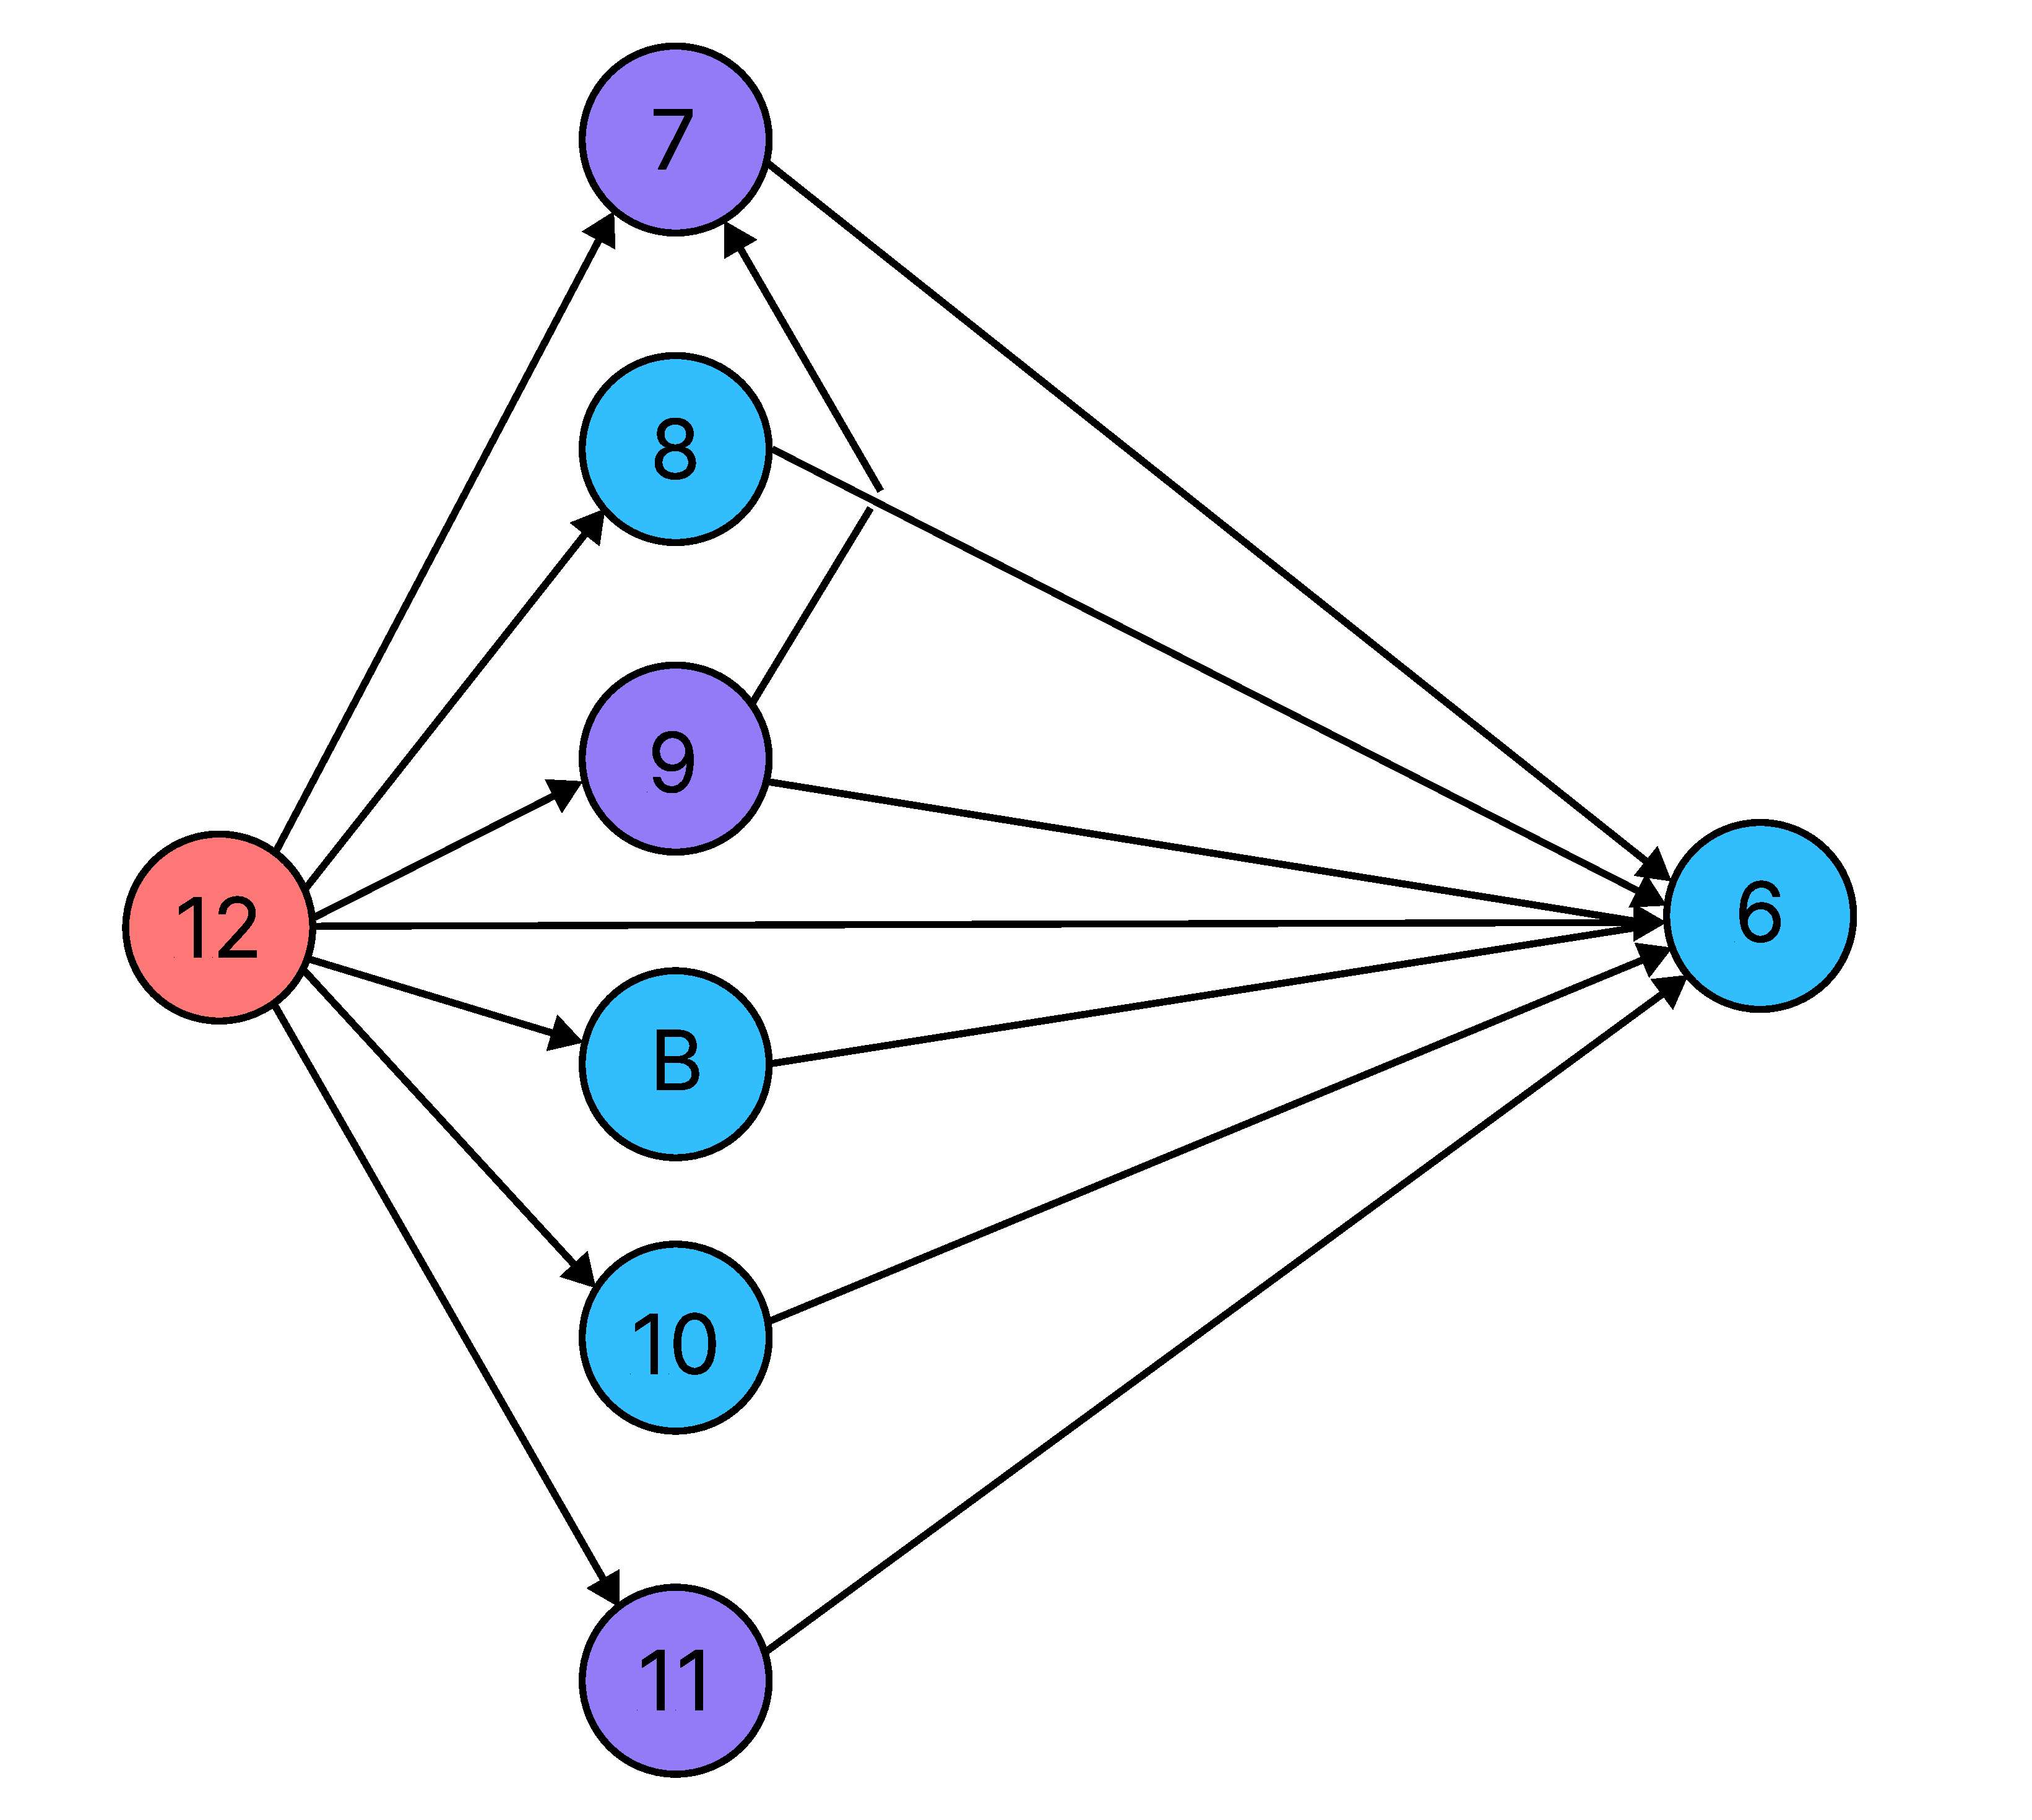
\includegraphics[width=1\textwidth]{sections/images/realated_works_graph}
    ~\caption{Related works graph.}\label{fig:related-works-graph}
\end{figure}
\begin{itemize}
    \item {\Large \textcircled{\normalsize 12}} This manuscript
    \item {\Large \textcircled{\normalsize 6}}
    In \textit{On the link between binomial theorem and discrete convolution}~\cite{on_the_link_between_binomial_theorem_and_discrete_convolution}:
    Let $\mathbf{P}^{m}_{b}(x)$ be a $2m+1$-degree polynomial in $x$ and $b \in \mathbb{R}$
    \[
        \mathbf{P}^{m}_{b}(x) = \sum_{k=0}^{b-1} \sum_{r=0}^{m} \mathbf{A}_{m,r} k^r (x-k)^r
    \]
    where $\mathbf{A}_{m,r}$ are real coefficients.
    In this manuscript, we introduce the polynomial $\mathbf{P}^{m}_{b}(x)$ and study its properties,
    establishing a polynomial identity for odd-powers in terms of this polynomial.
    Based on mentioned polynomial identity for odd-powers,
    we explore the connection between the Binomial theorem and discrete convolution of odd-powers,
    further extending this relation to the multinomial case.
    All findings are verified using Mathematica programs.
    \item {\Large \textcircled{\normalsize 7}}
    In \textit{A study on partial dynamic equation on time scales involving derivatives
    of polynomials}~\cite{study_on_partial_dynamic_eq_on_time_scales_with_poly_derivatives}:
    Extends the main results of {\Large \textcircled{\normalsize 6}} deriving and discussing
    an identity that connects the timescale derivative of odd-powered polynomial
    with partial derivatives of polynomial $\polynomialP{m}{b}{x}$ evaluated in particular points.
    For every $t\in\mathbb{T}_1$ and $(x,b) \in \Lambda^2$
    \[
        \frac{\Delta x^{2m+1}}{\Delta x}(t) =
        \frac{\partial P(m,b,x)}{\Delta x} (m, \sigma(t), t) +
        \frac{\partial P(m,b,x)}{\Delta b} (m, t, t)
    \]
    such that $\sigma(t) > t$ is forward jump operator.
    In addition, we discuss various derivative operators in the context of the partial cases of above equation,
    We show finite difference, classical derivative, $q-$derivative, $q-$power derivative on behalf of it.
    \item {\Large \textcircled{\normalsize 8}}
    In \textit{106.37 An unusual identity for odd-powers}~\cite{unusual_identity_for_odd_powers}:
    Explores and proves the partial case of {\Large \textcircled{\normalsize 6}}
    that is the polynomial identity for odd-powers
    \[
        n^{2m+1} = \sum_{k=1}^{n} \sum_{r=0}^{m} \mathbf{A}_{m,r} k^r (n-k)^r
    \]
    \item {\Large \textcircled{\normalsize 9}}
    In \textit{Another approach to get derivative of odd-power}~\cite{another_approach_to_get_derivative_of_odd_power}:
    Extends the results of {\Large \textcircled{\normalsize 6}} by providing a relation in terms of partial differential equations such that
    ordinary derivative of odd-power $2m+1$ can be reached in terms of partial derivative of the polynomial $\polynomialP{m}{b}{x}$.
    Let be a fixed point $v\in \mathbb{N}$, then ordinary derivative $\frac{d}{dx} g_v (u)$ of the odd-power function $g_v(x) = x^{2v + 1}$
    evaluate in point $u\in\mathbb{R}$ equals to partial derivative $(f_{v})^{'}_{x} (u, u)$ evaluate in point $(u, u)$ plus
    partial derivative $(f_{v})^{'}_{z} (u, u)$ evaluate in point $(u, u)$
    \begin{equation}
        \frac{d}{dx} g_v (u) = (f_{v})^{'}_{x} (u, u) + (f_{v})^{'}_{z} (u, u)
        \label{eq:odd-exponential-identity}
    \end{equation}
    where $f_{y} (x, z) = \sum_{k=1}^{z} \sum_{r=0}^{y} \coeffA{y}{r} k^r (x-k)^r = \polynomialP{y}{z}{x}$.
    \item {\Large \textcircled{\normalsize B}}
    In \textit{A two-sided Faulhaber-like formula involving Bernoulli polynomials}~\cite{barbero2020two}:
    Based on equation~\eqref{eq:rearranging-terms}, the authors give a new identity involving
    Bernoulli polynomials and combinatorial numbers that provides,
    in particular, the Faulhaber-like formula for sums of the form $1^m(n-1)^m + 2^m (n -2)^m + \cdots + (n - 1)^m 1^m$
    for positive integers $m$ and $n$.
    \item {\Large \textcircled{\normalsize 10}}
    In \textit{Polynomial identity involving Binomial Theorem and Faulhaber's formula}~\cite{polynomial_identity_with_binomial_theorem_and_faulhabers_formula}:
    proves that
    for every $n\geq 1, \; n,m\in\mathbb{N}$
    there are coefficients $\mathbf{A}_{m,0}, \mathbf{A}_{m,1}, \ldots, \mathbf{A}_{m,m}$ such that
    the polynomial identity holds
    \[
        n^{2m+1} = \sum_{k=1}^{n} \mathbf{A}_{m,0} k^0 (n-k)^0 + \mathbf{A}_{m,1}(n-k)^1
        + \cdots + \mathbf{A}_{m,m} k^m (n-k)^m
    \]
    which is a direct consequence of the definition of $\polynomialP{m}{b}{x}$ given in {\Large \textcircled{\normalsize 6}},
    reached by utilizing Binomial theorem and Faulhaber's formula.
    \item {\Large \textcircled{\normalsize 11}}
    In \textit{Finding the derivative of polynomials via double limit}~\cite{derivative_of_polynomials_via_double_limit}:
    By applying the results of {\Large \textcircled{\normalsize 6}} provides
    another perspective of ordinary derivatives of polynomials allowing expressing
    them via a double limit, because
    \begin{align*}
        \lim_{h \to 0} \polynomialP{m}{x+h}{x} = x^{2m+1}
    \end{align*}
    \item Three sequences were contributed to the
    OEIS~\cite{oeis_coefficients_u_m_l_k_defined_by_polynomial_identity_1, oeis_coefficients_u_m_l_k_defined_by_polynomial_identity_2, oeis_coefficients_u_m_l_k_defined_by_polynomial_identity_3}
    showing the coefficients of the polynomial $\polynomialP{m}{b}{x}$ having fixed points $m,b$ while $x\in\mathbb{R}$.
    \item OEIS sequences such that row sums give odd-powers~\cite{oeis_numerical_triangle_row_sums_give_cubes, oeis_numerical_triangle_row_sums_give_fifth_powers, oeis_numerical_triangle_row_sums_give_seventh_powers}.
    \item OEIS sequences related to the coefficients $\coeffA{m}{r}$~\cite{oeis_numerators_of_the_coefficient_a_m_r, oeis_denominators_of_the_coefficient_a_m_r}.
\end{itemize}
The node indexes in the related works graph are not random, persisting the same values as
these works have on my personal website
\begin{center}
    \href{https://kolosovpetro.github.io/math/}{\texttt{kolosovpetro.github.io/math}}
\end{center}

%
%
%    \section{Future research}\label{sec:future-research}
%    Several promising directions emerge from the findings of this manuscript:

\begin{itemize}
    \item \textbf{Integration into mathematical literature.}
    The identities presented in this work do not appear in standard mathematical references,
    despite their elementary nature and apparent classical flavor.
    Notably, related sequences are absent from major repositories such as the OEIS\@.
    Future work should investigate the originality of these results and aim to contextualize
    them within the broader mathematical framework.

    \item \textbf{Extension of approximation methods.}
    The approximation technique developed in~\cite{kolosov2025efficient} is generalizable
    to a broader class of polynomials.
    In particular, by leveraging the symmetry property~\eqref{prop:Tm-symmetry},
    one could explore alternative summation domains for the polynomials $P(m, X, N)$.

    \item \textbf{Combinatorial interpretation of $T_m(n,k)$.}
    The polynomial family $T_m(n,k)$, introduced in~\eqref{def:bivariate-sum-Tm},
    currently lacks a clear combinatorial interpretation.
    Understanding its structural or enumerative significance would deepen insight into
    the algebraic identities presented.

    \item \textbf{Connection with finite differences and derivatives.}
    The binomial form of the odd power identity~\eqref{prop:binomial-form} offers a mechanism
    to express both finite differences and classical derivatives of odd powers in terms
    of the coefficients $\coeffA{m}{r}$.

    \item \textbf{$q$-derivative representation.}
    The general identity~\eqref{theorem:odd-power-identity} also suggests a natural
    expression for $q$-derivatives via the coefficients $\coeffA{m}{r}$,
    potentially leading to a generalized notion of differentiation through limiting procedures.
\end{itemize}

%
%
%    \section{Conclusions}\label{sec:conclusions}
%    In this manuscript we have successfully provided a comprehensive historical survey
of the milestones and evolution of the polynomial $\polynomialP{m}{b}{x}$
as well as related works such that based onto, for instance various polynomial identities, differential equations etc.
In addition, future research directions are proposed and discussed.

%
%    \section*{Acknowledgements}
%    The author is grateful to Albert Tkaczyk for pointing out the idea of the general form of odd power identity,
and for providing examples of how to build and solve systems of linear equations to evaluate $\coeffA{m}{r}$.
The author is grateful to Max Alekseyev (George Washington University) for providing a valuable contribution
of recurrence relation for coefficients $\coeffA{m}{r}$.
The author is grateful to Markus Scheuer for his help in proving the identity~\eqref{eq:combinatorial-identity},
the proof is elegant and beautiful.
Finally, the author is grateful to OEIS editors for their valuable work during the sequences
related to this manuscript were submitted.


    \bibliographystyle{unsrt}
    \bibliography{surprising-polynomial-identities-classical-interpolation}

%    \noindent \textbf{Version:} \texttt{Local-0.1.0}
%    \\[1em]
%    \noindent \textbf{License:} This work is licensed under a
%    \href{https://creativecommons.org/licenses/by/4.0/}
%    {\texttt{Creative Commons Attribution 4.0 International License (CC BY 4.0)}}.

%    \section{Addendum 1: Examples of the polynomial \texorpdfstring{$\polynomialP{m}{b}{x}$}{P[m,b,x]}}
%    \label{sec:addendum-1}
%    \begin{equation*}
    \begin{split}
        \polynomialP{0}{b}{x}
        &=b \\
        \polynomialP{1}{b}{x}
        &=3 b^2 - 2 b^3 - 3 b x + 3 b^2 x \\
        \polynomialP{2}{b}{x}
        &=10 b^3 - 15 b^4 + 6 b^5- 15 b^2 x + 30 b^3 x - 15 b^4 x + 5 b x^2 - 15 b^2 x^2 + 10 b^3 x^2 \\
        \polynomialP{3}{b}{x}
        &=-7 b^2 + 28 b^3 - 70 b^5 + 70 b^6 - 20 b^7 + 7 b x - 42 b^2 x + 175 b^4 x - 210 b^5 x + 70 b^6 x \\
        &+ 14 b x^2 - 140 b^3 x^2 + 210 b^4 x^2 - 84 b^5 x^2 + 35 b^2 x^3 - 70 b^3 x^3 + 35 b^4 x^3 \\
        \polynomialP{4}{b}{x}
        &= -60 b^2 + 180 b^3 - 294 b^5 + 420 b^7 - 315 b^8 + 70 b^9 + 60 b x - 270 b^2 x + 735 b^4 x - 1470 b^6 x \\
        &+ 1260 b^7 x - 315 b^8 x + 90 b x^2 - 630 b^3 x^2 + 1890 b^5 x^2 - 1890 b^6 x^2 + 540 b^7 x^2 + 210 b^2 x^3 \\
        &- 1050 b^4 x^3 + 1260 b^5 x^3 - 420 b^6 x^3 - 21 b x^4 + 210 b^3 x^4 - 315 b^4 x^4 + 126 b^5 x^4\\
        \polynomialP{5}{b}{x}
        &= -693 b^2 + 2068 b^3 - 330 b^4 - 2640 b^5 + 2772 b^7 - 2310 b^9 + 1386 b^{10} - 252 b^{11} + 693 b x \\
        &- 3102 b^2 x + 660 b^3 x + 6600 b^4 x - 9702 b^6 x + 10395 b^8 x - 6930 b^9 x + 1386 b^{10} x + 1034 b x^2 \\
        &- 330 b^2 x^2 - 5940 b^3 x^2 + 12936 b^5 x^2 - 18480 b^7 x^2 + 13860 b^8 x^2 - 3080 b^9 x^2 + 2310 b^2 x^3 \\
        &- 8085 b^4 x^3 + 16170 b^6 x^3 - 13860 b^7 x^3 + 3465 b^8 x^3 - 330 b x^4 + 2310 b^3 x^4 - 6930 b^5 x^4 \\
        &+ 6930 b^6 x^4 - 1980 b^7 x^4 - 231 b^2 x^5 + 1155 b^4 x^5 - 1386 b^5 x^5 + 462 b^6 x^5 \\
        \polynomialP{6}{b}{x}
        &= -10920 b^2 + 33306 b^3 - 9009 b^4 - 36036 b^5 + 37752 b^7 - 22022 b^9 + 12012 b^{11} - 6006 b^{12} + 924 b^{13} \\
        &+ 10920 b x - 49959 b^2 x + 18018 b^3 x + 90090 b^4 x - 132132 b^6 x + 99099 b^8 x - 66066 b^{10} x + 36036 b^{11} x \\
        &- 6006 b^{12} x + 16653 b x^2 - 9009 b^2 x^2 - 84084 b^3 x^2 + 180180 b^5 x^2 - 180180 b^7 x^2 + 150150 b^9 x^2 \\
        &- 90090 b^{10} x^2 + 16380 b^{11} x^2 + 36036 b^2 x^3 - 120120 b^4 x^3 + 168168 b^6 x^3 - 180180 b^8 x^3 \\
        &+ 120120 b^9 x^3 - 24024 b^{10} x^3 - 6006 b x^4 + 40040 b^3 x^4 - 84084 b^5 x^4 + 120120 b^7 x^4 - 90090 b^8 x^4 \\
        &+ 20020 b^9 x^4 - 6006 b^2 x^5 + 21021 b^4 x^5 - 42042 b^6 x^5 + 36036 b^7 x^5 - 9009 b^8 x^5 + 286 b x^6 \\
        &- 2002 b^3 x^6 + 6006 b^5 x^6 - 6006 b^6 x^6 + 1716 b^7 x^6
    \end{split}
\end{equation*}

%
%
%    \section{Addendum 2: Derivation of the coefficients \texorpdfstring{$\coeffA{m}{r}$}{A[m,r]}}
%    \label{sec:addendum-2}
%    Consider the definition~\eqref{eq:definition_coefficient_a} of the coefficients $\coeffA{m}{r}$, it can be written as
\begin{equation*}
    \coeffA{m}{r} =
    \begin{cases}
    (2r+1)
        \binom{2r}{r}, & \text{if } r=m; \\
        \sum_{d \geq 2r+1}^{m} \coeffA{m}{d} \underbrace{(2r+1) \binom{2r}{r} \binom{d}{2r+1} \frac{(-1)^{d-1}}{d-r} \bernoulli{2d-2r}}_{T(d,r)}, & \text{if } 0 \leq r<m; \\
        0, & \text{if } r<0 \text{ or } r>m,
    \end{cases}
\end{equation*}
Therefore, let be a definition of the real coefficient $T(d,r)$
\begin{definition}
    Real coefficient $T(d,r)$
    \begin{equation*}
        T(d,r) = (2r+1) \binom{2r}{r} \binom{d}{2r+1} \frac{(-1)^{d-1}}{d-r} \bernoulli{2d-2r}
    \end{equation*}
\end{definition}
\begin{example}
    Let be $m=2$ so first we get $\coeffA{2}{2}$
    \begin{equation*}
        \coeffA{2}{2} = 5\binom{4}{2}=30
    \end{equation*}
    Then $\coeffA{2}{1} = 0$ because $\coeffA{m}{d}$ is zero in the range $m/2 \leq d < m$ means that zero for $d$
    in $1 \leq d < 2$.
    Finally, the coefficient $\coeffA{2}{0}$ is
    \begin{equation*}
        \begin{split}
            \coeffA{2}{0}
            = \sum_{d \geq 1}^{2} \coeffA{2}{d} \cdot T(d, 0)
            &= \coeffA{2}{1} \cdot T(1, 0) + \coeffA{2}{2} \cdot T(2, 0) \\
            &= 30 \cdot \frac{1}{30} = 1
        \end{split}
    \end{equation*}
\end{example}
\begin{example}
    Let be $m=3$ so that first we get $\coeffA{3}{3}$
    \begin{equation*}
        \coeffA{3}{3} = 7 \binom{6}{3}= 140
    \end{equation*}
    Then $\coeffA{3}{2} = 0$ because $\coeffA{m}{d}$ is zero in the range $m/2 \leq d < m$ means that zero for $d$
    in $2 \leq d < 3$.
    The $\coeffA{3}{1}$ coefficient is non-zero and calculated as
    \begin{equation*}
        \begin{split}
            \coeffA{3}{1} = \sum_{d \geq 3}^{3} \coeffA{3}{d} \cdot T(d,1) = \coeffA{3}{3} \cdot T(3,1)
            = 140 \cdot \left( -\frac{1}{10} \right) = -14
        \end{split}
    \end{equation*}
    Finally, the coefficient $\coeffA{3}{0}$ is
    \begin{equation*}
        \begin{split}
            \coeffA{3}{0}= \sum_{d \geq 1}^{3} \coeffA{3}{d} \cdot T(d,0)
            &= \coeffA{3}{1} \cdot T(1,0) + \coeffA{3}{2} \cdot T(2,0) + \coeffA{3}{3} \cdot T(3,0) \\
            &= -14 \cdot \frac{1}{6} + 140 \cdot \frac{1}{42} = 1
        \end{split}
    \end{equation*}
\end{example}
\begin{example}
    Let be $m=4$ so that first we get $\coeffA{4}{4}$
    \begin{equation*}
        \coeffA{4}{4} = 9 \binom{8}{4}= 630
    \end{equation*}
    Then $\coeffA{4}{3} = 0$ and $\coeffA{4}{2} = 0$
    because $\coeffA{m}{d}$ is zero in the range $m/2 \leq d < m$ means that zero for $d$ in $2 \leq d < 4$.
    The value of the coefficient $\coeffA{4}{1}$ is non-zero and calculated as
    \begin{equation*}
        \begin{split}
            \coeffA{4}{1}
            = \sum_{d \geq 3}^{4} \coeffA{4}{d} \cdot T(d,1)
            = \coeffA{4}{3} \cdot T(3,1) + \coeffA{4}{4} \cdot T(4,1)
            = 630 \cdot \left( -\frac{4}{21} \right)
            = -120
        \end{split}
    \end{equation*}
    Finally, the coefficient $\coeffA{4}{0}$ is
    \begin{equation*}
        \begin{split}
            \coeffA{4}{0}
            = \sum_{d \geq 1}^{4} \coeffA{4}{d} \cdot T(d, 0)
            = \coeffA{4}{1} \cdot T(1, 0) + \coeffA{4}{4} \cdot T(4, 0)
            = -120 \cdot \frac{1}{6} + 630 \cdot \frac{1}{30} = 1
        \end{split}
    \end{equation*}
\end{example}
\begin{example}
    Let be $m=5$ so that first we get $\coeffA{5}{5}$
    \begin{equation*}
        \coeffA{5}{5} = 11 \binom{10}{5}= 2772
    \end{equation*}
    Then $\coeffA{5}{4} = 0$ and $\coeffA{5}{3} = 0$
    because $\coeffA{m}{d}$ is zero in the range $m/2 \leq d < m$ means that zero for $d$ in $3 \leq d < 5$.
    The value of the coefficient $\coeffA{5}{2}$ is non-zero and calculated as
    \begin{equation*}
        \begin{split}
            \coeffA{5}{2}
            = \sum_{d \geq 5}^{5} \coeffA{5}{d} \cdot T(d,2) = \coeffA{5}{5} \cdot T(5,2) = 2772 \cdot \frac{5}{21} = 660
        \end{split}
    \end{equation*}
    The value of the coefficient $\coeffA{5}{1}$ is non-zero and calculated as
    \begin{equation*}
        \begin{split}
            \coeffA{5}{1}
            &= \sum_{d \geq 3}^{5} \coeffA{5}{d} \cdot T(d,1)
            = \coeffA{5}{3} \cdot T(3,1) + \coeffA{5}{4} \cdot T(4,1) + \coeffA{5}{5} \cdot T(5,1) \\
            &= 2772 \cdot \left( - \frac{1}{2} \right) = -1386
        \end{split}
    \end{equation*}
    Finally, the coefficient $\coeffA{5}{0}$ is
    \begin{equation*}
        \begin{split}
            \coeffA{5}{0}
            &= \sum_{d \geq 1}^{5} \coeffA{5}{d} \cdot T(d, 0)
            = \coeffA{5}{1} \cdot T(1, 0) + \coeffA{5}{2} \cdot T(2, 0) + \coeffA{5}{5} \cdot T(5, 0) \\
            &= -1386 \cdot \frac{1}{6} + 660 \cdot \frac{1}{30} + 2772 \cdot \frac{5}{66} = 1
        \end{split}
    \end{equation*}
\end{example}

%
%
%    \section{Addendum 3: Odd power identities}
%    \label{sec:addendum-3}
%    \begin{align*}
    n^3 &= \sum_{k=1}^{n} 6k(n-k) + 1 \\
    n^5 &= \sum_{k=1}^{n} 30k^2(n-k)^2 + 1 \\
    n^7 &= \sum_{k=1}^{n} 140 k^3 (n-k)^3 - 14k(n-k) + 1 \\
    n^9 &= \sum_{k=1}^{n} 630 k^4(n-k)^4 - 120k(n-k) + 1 \\
    n^{11} &= \sum_{k=1}^{n} 2772 k^5(n-k)^5 + 660 k^2(n-k)^2 - 1386k(n-k) + 1 \\
    n^{13} &= \sum_{k=1}^{n} 51480 k^7(n-k)^7 - 60060 k^3(n-k)^3 + 491400k^2(n-k)^{2} - 450054k(n-k) + 1 \\
\end{align*}


\end{document}
